

\documentclass[11pt]{beamer}

\usetheme{Madrid}
\usecolortheme{seahorse}
\setbeamertemplate{navigation symbols}{}

\usepackage[utf8]{inputenc}
\usepackage[T1]{fontenc}
\usepackage[ngerman,english]{babel}
\usepackage{amsmath,amssymb,bm,mathtools}
\usepackage{graphicx}
\usepackage{booktabs}
\usepackage{microtype}

\newcommand{\E}{\mathbb E}
\newcommand{\Var}{\operatorname{Var}}
\newcommand{\sigmoid}{\sigma}

\title[Spatial Poisson Fields]{From Point Events to Posterior Fields}
\author[T. Luhdo]{Toni Luhdo}
\institute[UP]{University of Potsdam}
\date[]{Research Group Seminar -- April 2026}

\AtBeginSection[]{
\begin{frame}{Outline}
\tableofcontents[currentsection]
\end{frame}
}

\begin{document}

\begin{frame}
\titlepage
\end{frame}

\begin{frame}{Roadmap}
\tableofcontents
\end{frame}

% -------------------------------------------------
\section{Motivation}

\begin{frame}{Spatial Event Data}
Typical examples:
\begin{itemize}
\item Earthquakes
\item Photon arrivals in imaging
\item Disease outbreaks
\item Crime hotspots
\end{itemize}

Observed data are often \textbf{point events} in space.

Goal: infer an underlying smooth intensity field.
\end{frame}

\begin{frame}{Synthetic Point Catalog}
\begin{center}
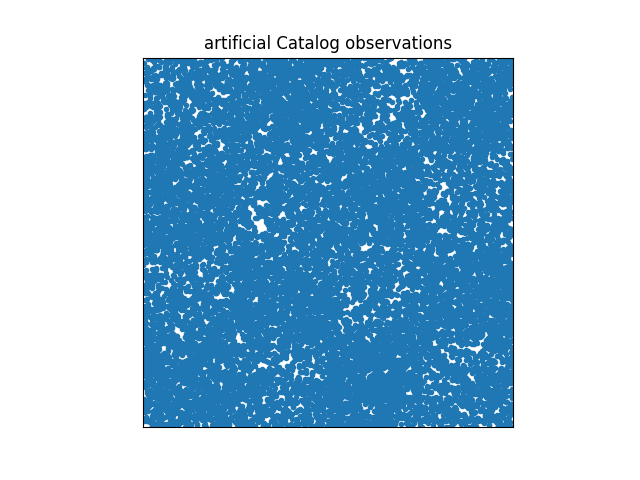
\includegraphics[width=0.72\textwidth]{figures/Figure_3.png}
\end{center}

We observe only events, not the true latent rate.
\end{frame}

% -------------------------------------------------
\section{Generative Model}

\begin{frame}{Latent Gaussian Field}
We introduce a latent spatial field:
\[
f \sim \mathcal N(\mu,\Sigma).
\]

The covariance matrix is generated from a spatial kernel:
\[
\Sigma_{ij}=K(x_i,x_j).
\]

Example:
\[
K(x_i,x_j)=v^2\exp\!\left(-\frac{\|x_i-x_j\|^2}{2\rho^2}\right)
\]

where

\begin{itemize}
\item $v^2$ = marginal prior variance
\item $\rho$ = correlation length
\item nearby cells are more strongly correlated
\end{itemize}

\medskip
Thus $\Sigma$ controls smoothness of the latent field.
\end{frame}

\begin{frame}{From Latent Field to Poisson Rate}
Rates must be positive. We use:
\[
\lambda_i = \lambda\,\sigmoid(f_i),
\qquad
\sigmoid(x)=\frac{1}{1+e^{-x}}
\]

Then:
\[
0 < \lambda_i < \lambda
\]

Advantages:
\begin{itemize}
\item positivity
\item bounded intensity
\item numerically stable inference
\end{itemize}
\end{frame}

\begin{frame}{Induced Local Priors on Intensity}
\begin{center}

\includegraphics[width=0.42\textwidth]{figures/Figure_1.png}
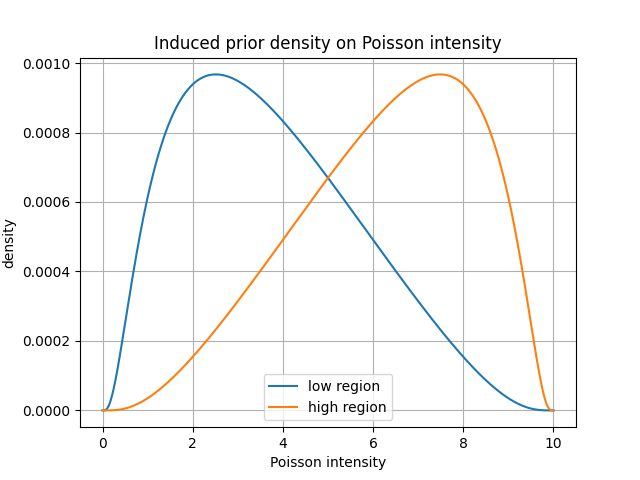
\includegraphics[width=0.42\textwidth]{figures/Figure_15.png}
\end{center}

The prior is Gaussian in the latent variable $f_i$, but the link function transforms it to the intensity scale:
\[
\lambda_i = \lambda\,\sigmoid(f_i).
\]

The two curves correspond to two different local prior means in latent space,
with the same one-dimensional variance:
% \[
% f_i \sim \mathcal N(\mu_{\mathrm{low}},v^2),
% \qquad
% f_i \sim \mathcal N(\mu_{\mathrm{high}},v^2).
% \]
\[
f_i \sim \mathcal N(\mu,v^2),
\]
\end{frame}

\begin{frame}{Synthetic Example: Structured Rate Field}
\begin{center}
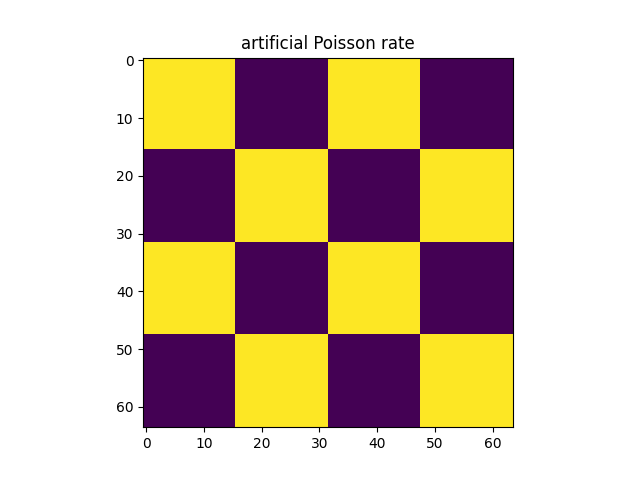
\includegraphics[width=0.61\textwidth]{figures/Figure_2.png}
\end{center}

We use the same checkerboard structure with two different contrast settings:
\[
\begin{array}{c|ccc}
& \lambda_{\mathrm{low}} & \lambda_{\mathrm{high}} & \lambda \\
\hline
\text{Example I} & 4.5 & 5.5 & 10 \\
\text{Example II} & 3.5 & 6.5 & 10
\end{array}
\]
\end{frame}


\begin{frame}{Discretization: From Point Events to Counts}
After discretization into grid cells:
\[
n_i = \#\{\text{events in cell } i\},
\qquad
n_i \sim \operatorname{Poisson}(\lambda_i)
\]
\vspace*{-15mm}
\begin{columns}[T]
    \begin{column}{0.49\textwidth}
    \begin{center}
    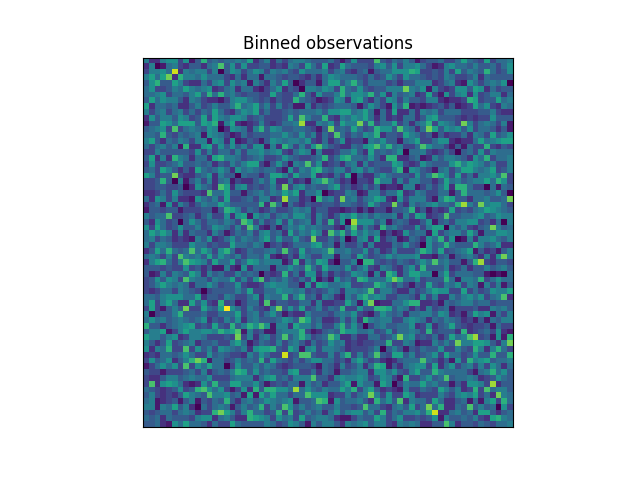
\includegraphics[width=\textwidth]{figures/Figure_11.png}
    \end{center}
    \end{column}
    \begin{column}{0.49\textwidth}
    \begin{center}
    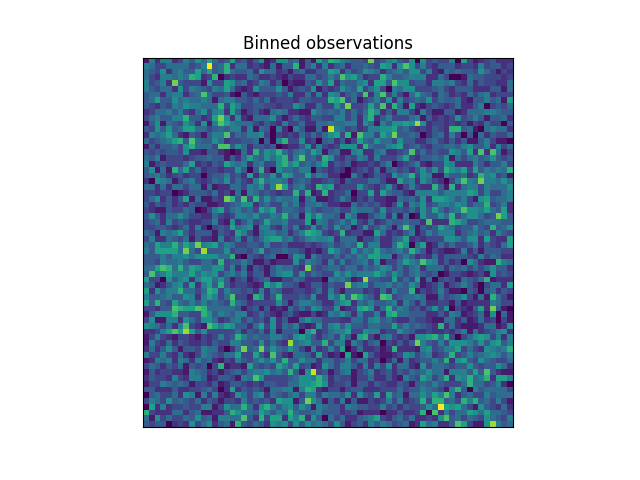
\includegraphics[width=\textwidth]{figures/Figure_4.png}
    \end{center}
    \end{column}
\end{columns}
\vspace*{-1mm}
The observations are discrete and noisy; the latent rate field is not observed.\\
\vspace*{2mm}
The generative model is now clear, but inference is not straightforward:\\
the Poisson--sigmoid likelihood is not conjugate to the Gaussian prior.
\end{frame}


% -------------------------------------------------
\section{Bayesian Inference}

\begin{frame}{Posterior Target}
We observe counts on grid cells and model
\[
n_i \mid f_i \sim \operatorname{Poisson}(\lambda\sigmoid(f_i)),
\qquad
f \sim \mathcal N(\mu,\Sigma).
\]

The posterior target is
\[
p(f\mid n) \propto p(n\mid f)\,p(f).
\]

The log-likelihood is, up to constants independent of $f$,
\[
\ell(f)=
\sum_i \left(
 n_i\log\sigmoid(f_i)
 - \lambda\sigmoid(f_i)
\right).
\]

\medskip
\textbf{Obstacle:} the Poisson--sigmoid likelihood is not conjugate to the Gaussian prior.
\end{frame}

\begin{frame}{Poisson Splitting: From Poisson to Logistic Form}
The exponential part can be rewritten as
\[
e^{-\lambda\sigmoid(f_i)}
=
e^{-\lambda}\,e^{\lambda\sigmoid(-f_i)}.
\]

Expanding the second exponential suggests latent counts
\[
k_i\mid f_i \sim \operatorname{Poisson}(\lambda\sigmoid(-f_i)).
\]

Together with the observed counts this gives the augmented likelihood
\[
p(n_i,k_i\mid f_i)
\propto
\left(\sigmoid(f_i)\right)^{n_i}
\left(\sigmoid(-f_i)\right)^{k_i}
=
\frac{e^{n_i f_i}}{(1+e^{f_i})^{n_i+k_i}}.
\]

\medskip
So the Poisson model is transformed into a logistic form.
\end{frame}

\begin{frame}{P\'olya--Gamma Augmentation}
Define
\[
b_i=n_i+k_i,
\qquad
\kappa_i=\frac{n_i-k_i}{2}.
\]

The augmented likelihood has the standard P\'olya--Gamma form
\[
\frac{e^{n_i f_i}}{(1+e^{f_i})^{b_i}}
\propto
\int_0^\infty
\exp\left(
-\frac12\omega_i f_i^2 + \kappa_i f_i
\right)
p(\omega_i\mid b_i,0)\,d\omega_i.
\]

Equivalently, in the Gibbs sampler we draw
\[
\omega_i\mid f_i,b_i \sim PG(b_i,f_i).
\]

\medskip
\textbf{Key point:} conditional on $\omega$, the likelihood is quadratic in $f$.
\end{frame}

\begin{frame}{Gaussian Update and Cholesky Sampling}
Combining the quadratic likelihood with the Gaussian prior gives
\[
\log p(f\mid n,k,\omega)
=
-\frac12 f^\top Qf+f^\top h+c,
\]
with
\[
Q=\Sigma^{-1}+\Omega,
\qquad
h=\Sigma^{-1}\mu+\kappa,
\qquad
\Omega=\operatorname{diag}(\omega_1,\dots,\omega_N).
\]

Thus
\[
f\mid n,k,\omega \sim \mathcal N(m,Q^{-1}),
\qquad
m=Q^{-1}h.
\]

In practice we do not compute $Q^{-1}$ explicitly. We use
\[
Q=LL^\top
\]
and solve triangular systems.
\end{frame}

% -------------------------------------------------
\section{Results}

\begin{frame}{Gaussian First Guess}
\begin{columns}[T]
\begin{column}{0.45\textwidth}
\begin{center}
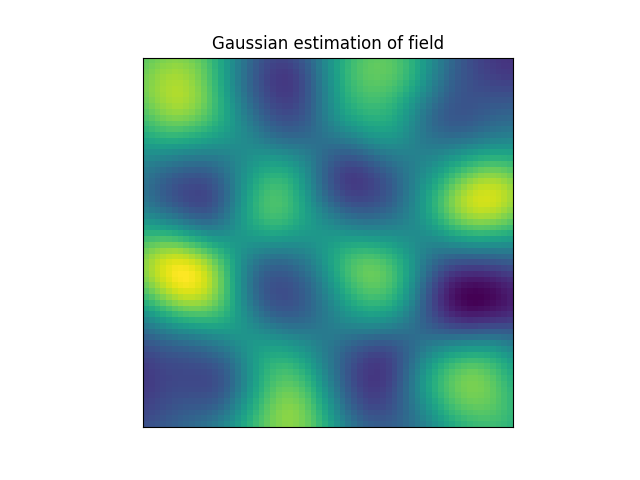
\includegraphics[width=\textwidth]{figures/Figure_5.png}
\end{center}
\end{column}
\begin{column}{0.55\textwidth}
\small
\begin{itemize}
\item Construct a pixelwise rate proxy from the observed counts:
\[
\tilde\lambda_i=\operatorname{clip}(n_i+1).
\]
\item Map it back to the latent scale:
\[
\tilde f_i=\sigmoid^{-1}\!\left(\frac{\tilde\lambda_i}{\lambda}\right).
\]
\end{itemize}
\end{column}
\end{columns}
\begin{itemize}
\item Approximate local uncertainty by error propagation:
\[
s_i^2\approx\frac{\tilde\lambda_i}{\left(\frac{d\lambda_i}{df_i}\right)^2}.
\]
\item Combine this noisy proxy with the Gaussian prior to obtain a smoothed initialization.
\end{itemize}
\end{frame}

\begin{frame}{Posterior Samples}
\begin{center}
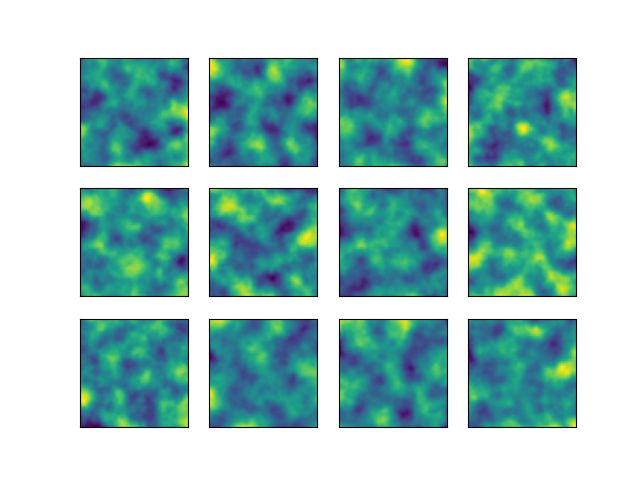
\includegraphics[width=0.82\textwidth]{figures/Figure_6.png}
\end{center}
\end{frame}

\begin{frame}{Posterior Mean Reconstruction: Example I}
Recovered spatial structure from event data.
The posterior mean is smoother than the discrete observations and reflects the spatial prior.

\begin{center}
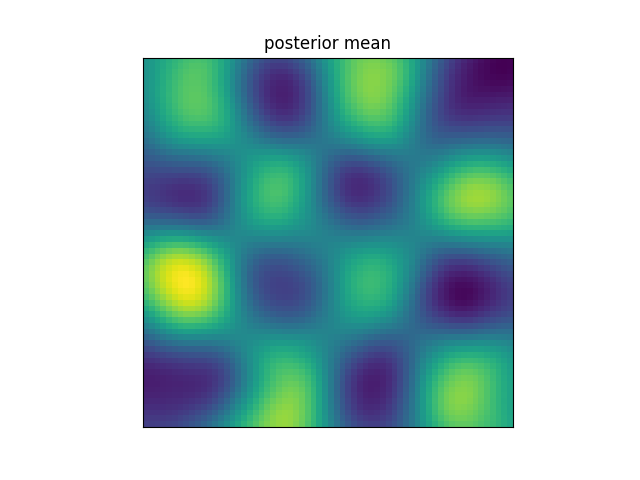
\includegraphics[width=0.72\textwidth]{figures/Figure_7.png}
\end{center}

\end{frame}

% \begin{frame}{Posterior Mean Reconstruction: Example II}
% The posterior mean is smoother than the discrete observations and reflects the spatial prior.
% \begin{center}
% 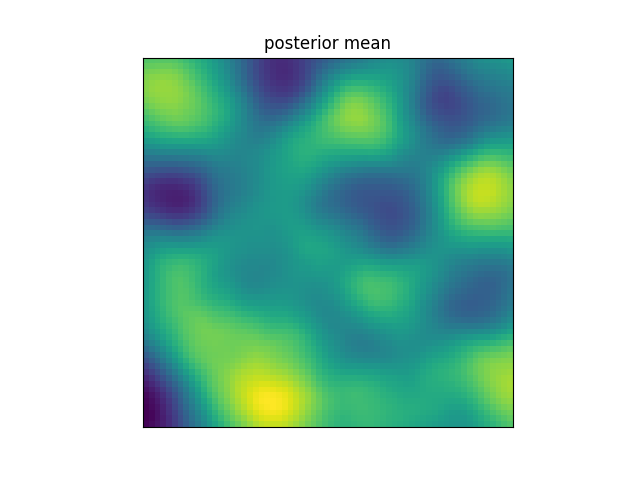
\includegraphics[width=0.72\textwidth]{figures/Figure_14.png}
% \end{center}
% \end{frame}

\begin{frame}{Comparing the Two Synthetic Examples}
Example I has moderate contrast $(4.5,5.5)$, whereas Example II has stronger contrast $(3.5,6.5)$. Both are reconstructed using the same latent Gaussian Poisson model.
\begin{columns}[T]
\begin{column}{0.52\textwidth}
\begin{center}
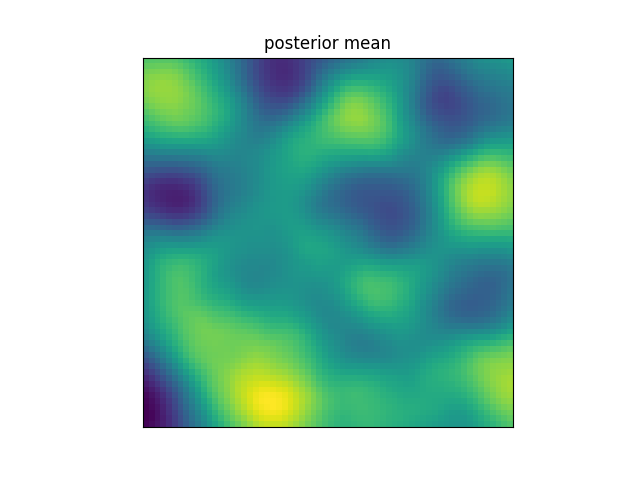
\includegraphics[width=\textwidth]{figures/Figure_14.png}

\scriptsize posterior mean, example I
\end{center}
\end{column}
\begin{column}{0.52\textwidth}
\begin{center}
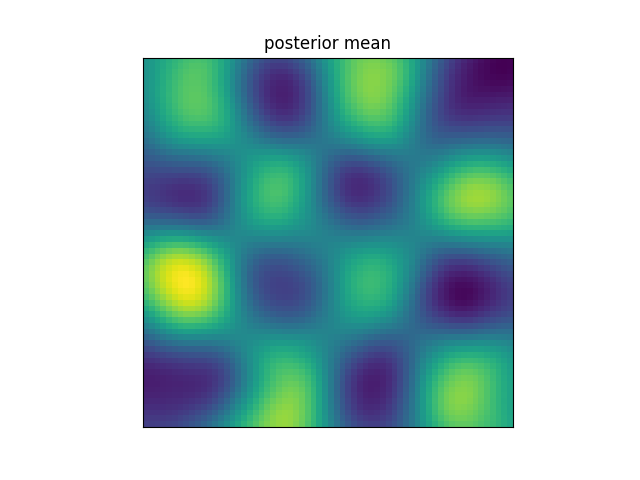
\includegraphics[width=\textwidth]{figures/Figure_7.png}

\scriptsize posterior mean, example II
\end{center}
\end{column}
\end{columns}

\end{frame}

% -------------------------------------------------
\section{Takeaways}

\begin{frame}{Takeaways}
\begin{itemize}
\item Point events can be modeled via latent spatial Poisson fields.
\item A Gaussian prior on $f$ induces flexible rate priors.
\item Poisson splitting converts the model into a logistic form.
\item P\'olya--Gamma augmentation then restores conditional Gaussian structure.
\item Gibbs sampling becomes efficient via Cholesky updates.
% \item The framework extends naturally to real earthquake data and adaptive grids.
\end{itemize}
\end{frame}


\begin{frame}{Outlook}
Future directions:
\begin{itemize}
\item Quadtree / adaptive grids
\item Sparse precision matrices
\item Nonstationary covariance kernels
\item Real earthquake catalogs
\item Spatio-temporal extensions
\end{itemize}
\end{frame}

\begin{frame}{Limitations of the Sigmoid Link}
The sigmoid link is useful because it guarantees positivity and gives a tractable P\'olya--Gamma Gibbs sampler.

\medskip
However, it also introduces limitations:
\begin{itemize}
\item the intensity is bounded by the fixed scale parameter $\lambda$,
\[
0<\lambda_i<\lambda,
\]
\item large positive values of $f_i$ are compressed due to saturation,
\item the P\'olya--Gamma variables change in every iteration, so the Gaussian update requires repeated linear algebra,
\item the upper bound may be restrictive for data sets with strongly varying event rates.
\end{itemize}

\medskip
This motivates considering alternative positive link functions.
\end{frame}

\begin{frame}{Beyond the Sigmoid Link}
A natural next question is:
\[
\text{Can we keep positivity while avoiding the fixed upper bound?}
\]

\medskip
One possible alternative is the softplus / soft-ramp link:
\[
\lambda_i = \log(1+e^{f_i}).
\]

\medskip
It remains positive, but grows approximately linearly for large $f_i$.

\begin{block}{Next part}
Cristina presents an alternative inference strategy based on this softer, unbounded link function.
\end{block}
\end{frame}

\begin{frame}{Thank you}
\begin{center}
\Large Thank you for your attention!\\[1em]
Questions?
\end{center}
\end{frame}

% -------------------------------------------------
\appendix
\section{Appendix}

\begin{frame}{Appendix: Synthetic Example II -- Event Catalog}
\begin{center}
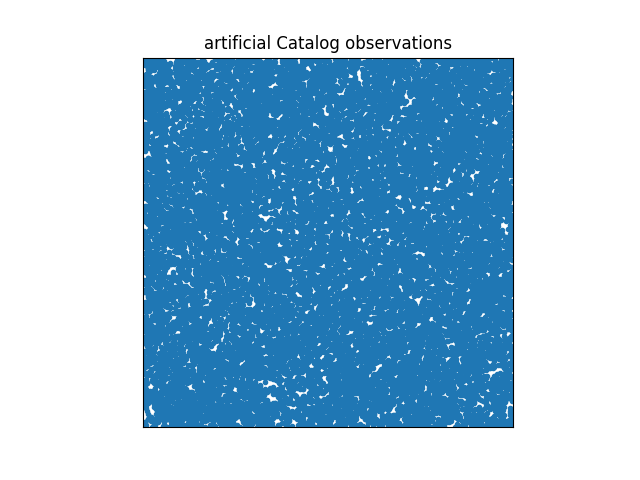
\includegraphics[width=0.72\textwidth]{figures/Figure_10.png}
\end{center}
\end{frame}

\begin{frame}{Appendix: Synthetic Example II -- Gaussian First Guess}
\begin{center}
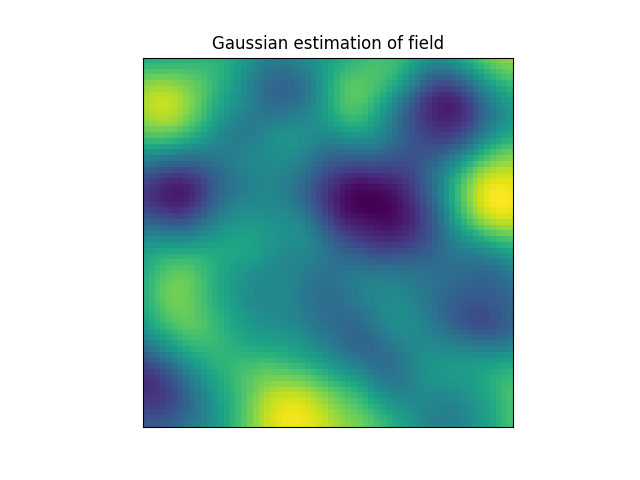
\includegraphics[width=0.72\textwidth]{figures/Figure_12.png}
\end{center}
\end{frame}

\begin{frame}{Appendix: Synthetic Example II -- Posterior Samples}
\begin{center}
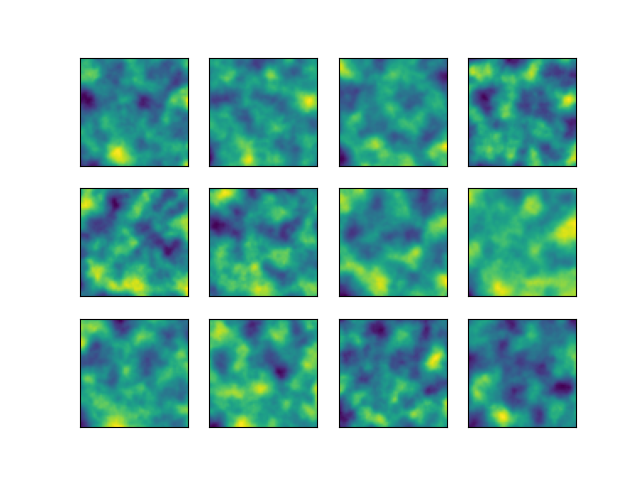
\includegraphics[width=0.82\textwidth]{figures/Figure_13.png}
\end{center}
\end{frame}

\begin{frame}{Appendix: Real Earthquake Data}

Possible discussion points:
\begin{itemize}
\item real point process data
\item spatially varying seismic activity
\item comparison with synthetic experiments
\end{itemize}
\end{frame}

\begin{frame}{Appendix: Adaptive Grid / Quadtree}

Possible discussion points:
\begin{itemize}
\item more cells where the data are dense
\item fewer cells where the data are sparse
\item rates must be interpreted relative to cell area
\end{itemize}
\end{frame}

\end{document}